\documentclass{article}
\usepackage[utf8]{inputenc}
\usepackage[italian]{babel}
\usepackage{natbib}
\usepackage{graphicx}
\usepackage[table,xcdraw]{xcolor}
\usepackage{listings}
\usepackage{amsmath}
\usepackage{minted}
\usepackage{amsthm}
\usepackage{enumitem}
\usepackage{color}
\usepackage[hidelinks]{hyperref}

\newcommand{\commonCrawlFilesTable}[0]{
    \renewcommand\arraystretch{1.2}
    % Please add the following required packages to your document preamble:
    % \usepackage{graphicx}
    % \usepackage[table,xcdraw]{xcolor}
    % If you use beamer only pass "xcolor=table" option, i.e. \documentclass[xcolor=table]{beamer}
    \begin{table}[h]
    \resizebox{\textwidth}{!}{%
    \begin{tabular}{lllr}
    \rowcolor[HTML]{C0C0C0} 
    Tipo File                                                          & Descrizione                                                                                                                                              & \#Files & \begin{tabular}[c]{@{}r@{}}Dim.dei file\\ compressi\end{tabular} \\ \hline
    \rowcolor[HTML]{EFEFEF} 
    Segments                                                           &                                                                                                                                                          & 100     &                                                                   \\
    WARC files                                                         & Dati grezzi generati dal Crawler                                                                                                                         & 64000   & 59.86 TiB                                                         \\
    \rowcolor[HTML]{EFEFEF} 
    WAT files                                                          & \begin{tabular}[c]{@{}l@{}}Contengono meta-dati relativi ai record nei \\ file WARC\end{tabular}                                                          & 64000   & 18.23 TiB                                                         \\
    WET files                                                          & \begin{tabular}[c]{@{}l@{}}Contengono solo testo semplice estratto \\ dai WARC\end{tabular}                                                              & 64000   & 7.62 TiB                                                          \\
    \rowcolor[HTML]{EFEFEF} 
    Robots.txt files                                                   & \begin{tabular}[c]{@{}l@{}}Files Robot.txt richiesti ai vari siti analizzati \\ (consentono al Crawler di scansionare \\ meglio i siti web)\end{tabular} & 64000   & 170 GiB                                                          \\
    \begin{tabular}[c]{@{}l@{}}Non-200 \\ responses files\end{tabular} & \begin{tabular}[c]{@{}l@{}}Risposte del server con HTTP status code \\ diverso da 200 (404, redirects, ecc.)\end{tabular}                                & 64000   & 1.79 TiB                                                          \\
    \rowcolor[HTML]{EFEFEF} 
    URL index files                                                    & \begin{tabular}[c]{@{}l@{}}Indice degli url analizzati, completo di utili \\ informazioni aggiuntive\end{tabular}                                        & 302     & 210 GiB                                                         
    \end{tabular}%
    }
    \end{table}
    \renewcommand\arraystretch{1.0}
}

%TOTALE: 88791
%tick: 49668
%x: 5371
%plus: 14058
%minus: 14941
%divided: 4753
\newcommand{\printHistogram}[0]{
    %\pgfplotsset{scaled y ticks=false}
    \begin{tikzpicture}
    \begin{axis}[
        symbolic x coords={\imgtick{},\imgx{},\imgplus{},\imgminus{},\imgdivided{}}, 
        ylabel = {occorrenze ($\cdot 10^3$)}, 
        xlabel = {Accuratezza dei risultati}, 
        xtick=data]
        
        \addplot[ybar,fill=white] coordinates {
            (\imgtick{}, 49.668)
            (\imgx{}, 5.371)
            (\imgplus{}, 14.058)
            (\imgminus{}, 14.941)
            (\imgdivided{}, 4.753)
        };
    \end{axis}
    \end{tikzpicture}
}

\newcommand{\printTimeGraph}[0]{
    \begin{tikzpicture}
    \begin{axis}[
      %ymin=20,
      %ymax=90,
      %width=15cm,
      %height=7cm,
      ylabel={tempo (minuti)},
      xlabel={\#files WET analizzati},
      %xticklabels={,2,4,6,8,10}, 
      legend style={at={(0.13,0.83)},
      anchor=west, legend columns=-1, font=\small},
      legend cell align=left,
      xtick=data
     ]

    \addlegendentry{abc}

    \addplot[blue, mark=+] coordinates {
        (2, 1.23)
        (4, 2.32)
        (6, 3.23)
        (8, 4.32)
        (10, 5.45)
    };
    
    \addplot[gray, mark=] coordinates {
        (2, 1.23)
        (4, 2.46)
        (6, 3.69)
        (8, 4.92)
        (10, 6.15)
    };
    \end{axis}
    \end{tikzpicture}
}

\setlist[itemize,1]{label=$\--$}

% ------------------- COMMANDS
\newcommand{\py}{Python }
\newcommand{\pycode}[1]{\textit{#1}}
\newcommand{\filename}[1]{\textit{#1}}
\newcommand{\function}[1]{\textit{#1}}
\newcommand{\command}[1]{\texttt{#1}}
%\newcommand{\path}[1]{\textit{#1}} #already defined

% ------------------- ENVIROMENTS AND THEOREMS
\newtheorem*{definition}{Definizione}

\title{Relazione Progetto Big Data\\Analisi della lingua di pagine html}
\author{Crosara Marco VR434403}
\date{Marzo 2019 / Aprile 2019}

\begin{document}

\maketitle
\thispagestyle{empty}

\vspace{\fill}

\begin{center}
  UNIVERSITÀ DEGLI STUDI DI VERONA\\
Anno Accademico 2018/2019
\end{center}

\newpage

%Indice
\tableofcontents
\thispagestyle{empty}

\newpage

%\addtocounter{section}{-1}

%  _____ _   _ _______ _____   ____  _____  _    _ ___________ ____  _   _ ______ 
% |_   _| \ | |__   __|  __ \ / __ \|  __ \| |  | |___  /_   _/ __ \| \ | |  ____|
%   | | |  \| |  | |  | |__) | |  | | |  | | |  | |  / /  | || |  | |  \| | |__   
%   | | | . ` |  | |  |  _  /| |  | | |  | | |  | | / /   | || |  | | . ` |  __|  
%  _| |_| |\  |  | |  | | \ \| |__| | |__| | |__| |/ /__ _| || |__| | |\  | |____ 
% |_____|_| \_|  |_|  |_|  \_\\____/|_____/ \____//_____|_____\____/|_| \_|______|

\section{Introduzione}

Il progetto è partito dalla curiosità di analizzare un grosso quantitativo di pagine web con lo scopo di farne in qualche modo categorizzazione. Come punto di partenza si è scelto di cercare un dataset opportuno a questo tipo di analisi, dopo una ricerca approfondita è stato scelto Common Crawl\cite{commoncrawl}: una enorme collezione di pagine dati in formato `raw', da cui sono stati estratti metadati e testo semplice. Tutti i dati in formato non elaborato sono raccolti mediante l'uso di un Crawler che esegue la scansione del web.

\begin{definition}
Il Crawler, comunemente chiamato anche Spider o Bot, è un software/script che ha lo scopo di scansionare dei dati. Tale termine viene tipicamente associato alla scansione di pagine web oppure di database con il fine di estrapolarne i contenuti. In particolare nella SEO il Crawler viene associato allo spider di Google. In realtà il crawling è una delle fasi per l’indicizzazione dei siti nella SERP(Search Engine Results Page), la pagina dei risultati di un motore di ricerca.
\end{definition}

Di seguito una tabella presente anche sulla pagina web di Common Crawl, utile per capire i diversi formati a disposizione degli utenti per la consultazione del dataset.

\commonCrawlFilesTable

\section{Obbiettivi del progetto}

\section{Struttura generale dell'analizzatore}

\section{Funzionamento e implementazione moduli}
\subsection{Parte 1}
\subsection{Parte 2}
\subsection{Parte 3}

\section{Test e Risultati Finali}
\subsection{Test su Docker-Cloudera}
\subsection{Test su cluster reale}


%  ________   __ _____   __ 
% |  ____\ \ / // ____| /_ |
% | |__   \ V /| (___    | |
% |  __|   > <  \___ \   | |
% | |____ / . \ ____) |  | |
% |______/_/ \_\_____/   |_|
% --------------- ESERCIZIO 1
%\section{Esercizio 1}

%\subsection{File dell'esercizio}
\begin{itemize}
    \item \filename{codicefiscale.py} : programma visto a lezione per il calcolo del codice fiscale 
    \item \filename{codicefiscale-test.py} : file con gli unit test
    \item \filename{.coverage} : risultati coverage
\end{itemize}

%\subsection{Considerazioni}
Il codice di \filename{codicefiscale.py} è quello visto a lezione, tuttavia è leggermente modificato poiché ne è stato fatto il porting del codice da \py 2 a \py 3. Il codice presenta degli errori che sono già stati riscontrati durante la lezione: ad esempio vi sono problemi se il cognome è troppo corto, il nome è troppo lungo o contiene uno spazio, oppure se la persona è nata il giorno 31 di qualsiasi mese.

%\subsection{Unit Testing}
\'E stato realizzato il file di unit testing \filename{codicefiscale-test.py} che fa il testing del \function{main} e di tutte le procedure ausiliarie: \function{estrai\_nome\_cognome}, \function{genera\_mese}, \function{codice\_comune}, \function{genera\_giorno}, \function{genera\_codice\_controllo}.

Gli unit test da implementare sono pochi poiché fin da subito si notano dei risultati discrepanti sull'output delle procedure che permettono di dichiarare il software come non corretto.
Gli unit test test implementati che vengono `falliti' sono 5.

I test presenti sul file consentono comunque di ottenere il 100\% della copertura. \'E stato aggiunto il flag \pycode{\#pragma: no cover} sul costrutto if relativo alla distinzione del file eseguito come script a se stante o richiamato come modulo, infatti tale ramo di esecuzione non risulta utile ai fini della verifica di copertura.

A seguito i risultati sulla verifica di copertura 100\% del codice.
\begin{minted}{bash}
mark@mark-XPS:~/.../progetto-finale/1$ python3-coverage report -m
Name                    Stmts   Miss  Cover   Missing
-----------------------------------------------------
codicefiscale-test.py      59      0   100%
codicefiscale.py           72      0   100%
-----------------------------------------------------
TOTAL                     131      0   100%
\end{minted}

L'esercizio si può considerare svolto con successo poiché si è riusciti tramite i test a dimostrare che il programma \filename{codicefiscale.py} è errato. Prima di svolgere ulteriori test per rilevare eventuali altri errori bisognerebbe correggere le procedure errate (non richiesto dalla consegna) e successivamente effettuare nuovi test su queste ultime. Siamo infine stati in grado di raggiungere la coverage 100\%.



\section{Considerazioni conclusive}

In alcuni esercizi si sarebbe potuto discutere l'utilizzo di \command{ltrace} anziché \command{strace} tuttavia abbiamo preferito il primo per comodità e continuità di utilizzo.

A riguardo degli esercizi 5a e 5b: \filename{AnalyzerPathAccess.java} e \filename{AnalyzerMemoryAccess.java} sono programmi pressoché uguali, infatti entrambi svolgono la funzione di ricerca di particolari log offerti da strace. Si sarebbe quindi potuto realizzare un unico programma di analisi per gli esercizi 5a e 5b oppure realizzare una libreria con le funzioni comuni, questo non è stato fatto per una logica di separazione degli esercizi.

%\begin{figure}[h!]
%\centering
%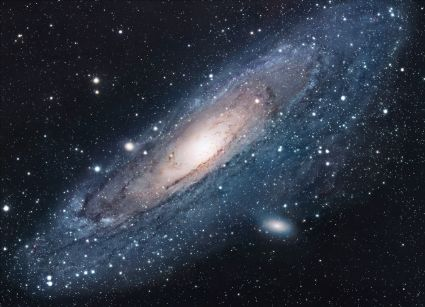
\includegraphics[scale=1.7]{universe}
%\caption{The Universe}
%\label{fig:universe}
%\end{figure}

\newpage

%bibliografia
\bibliographystyle{plain}
\bibliography{references}

%bibliografia senza citazioni
\nocite{strace}
\nocite{crawler}

\end{document}